\section{Aplicativo Web}
\label{Sec:5-aplicativo-web}

O componente de software teve como base de implementação o framework para desenvolvimento web Django, para a linguagem python. Várias funções especificadas anteriormente possuem uma certa interdependência entre elas, por exemplo, a função Criar Meta necessita que a função Criar Equipamento esteja previamente desenvolvida. Para isso, adotou-se a seguinte ordem de implementação de funções:

\begin{enumerate}
	\item{Fazer cadastro}
	\item{Fazer login}
	\item{Fazer logout}
	\item{Recuperar senha}
	\item{Criar equipamento}
	\item{Editar equipamento}
	\item{Remover equipamento}
	\item{Criar meta}
	\item{Editar meta}
	\item{Remover meta}
	\item{Atualizar taxas da AES}
	\item{Detectar sensores}
	\item{Editar sensor}
	\item{Remover sensor}
	\item{Configurar sistema}
	\item{Criar consumo}
	\item{Importar consumo}
	\item{Exportar consumo}
	\item{Visualizar consumo}
\end{enumerate}

\subsection{Telas principais}
%\subsubsection{Fazer login}
%Ao acessar o sistema pela url raiz, a tela AAAAA está disponível para o usuário. Caso ele possua login basta preencher o formulário e clicar em "Entrar". Caso contrário, o usuário deve clicar no botão "Cadastrar" para ser redirecionado à sua tela de cadastro.
%\subsubsection{Fazer cadastro}
%\subsubsection{Tela principal}
%\subsubsection{Criar equipamento}
\subsubsection{Listagem de equipamentos}
\begin{figure}[H]
\centering
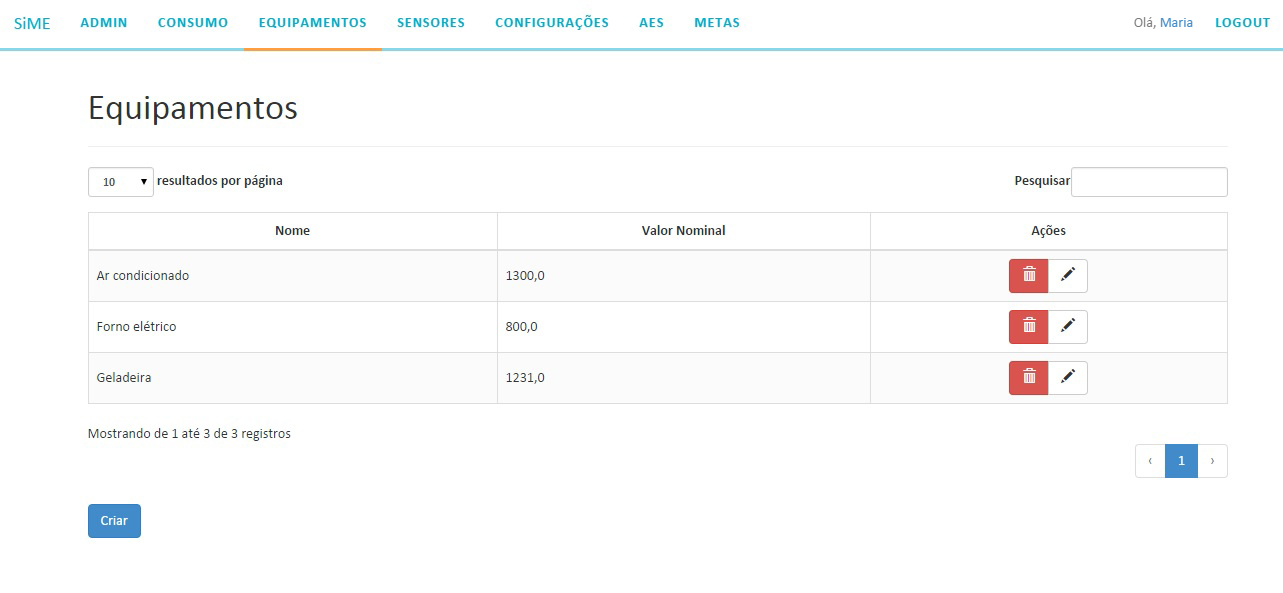
\includegraphics[width=1\textwidth]{figuras/equipamentos_list.jpg}
\caption{\label{fig:telas-equipamentos-list} Listagem de equipamentos}
\end{figure}

\subsubsection{Criar meta}
\begin{figure}[H]
\centering
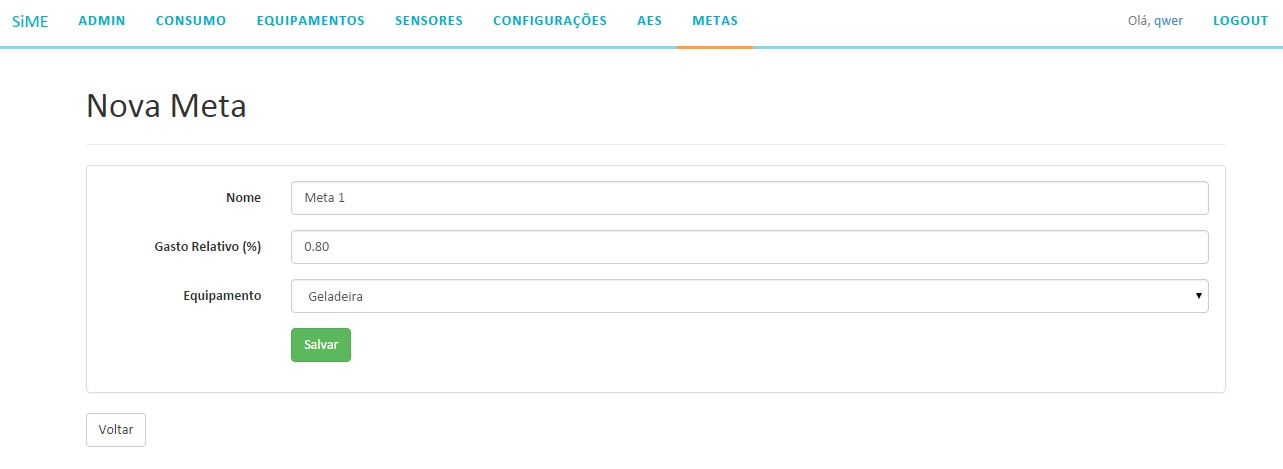
\includegraphics[width=1\textwidth]{figuras/meta.jpg}
\caption{\label{fig:telas-metas-create} Criar meta}
\end{figure}

\subsubsection{AES}
\begin{figure}[H]
\centering
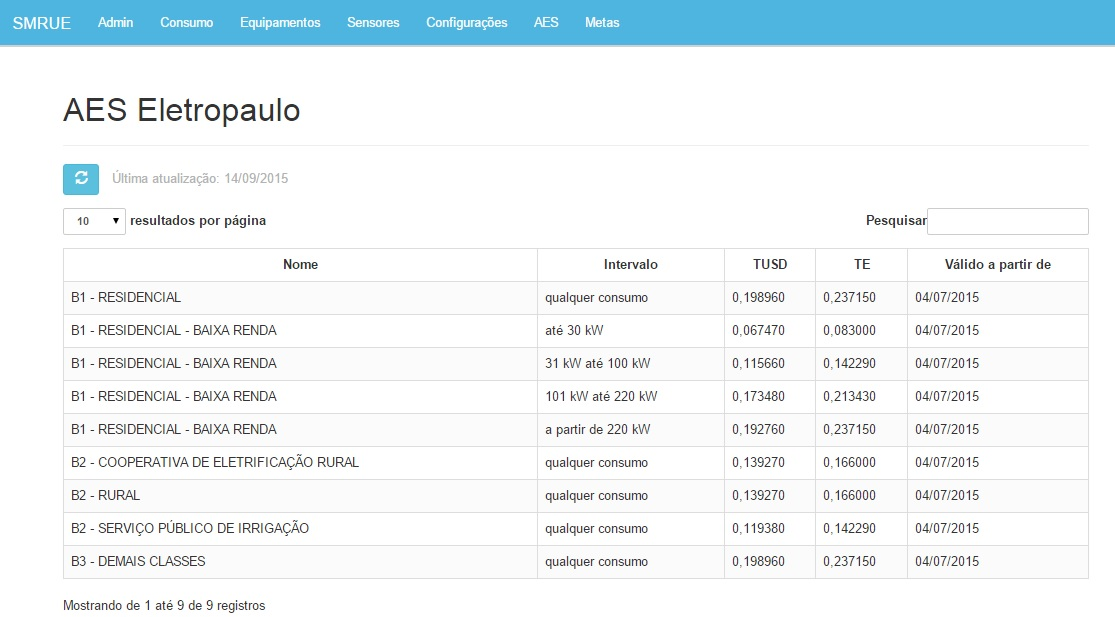
\includegraphics[width=1\textwidth]{figuras/aes.jpg}
\caption{\label{fig:telas-aes} AES}
\end{figure}

%\subsubsection{Listagem de sensores}
\subsubsection{Configurar sistema}
\begin{figure}[H]
\centering
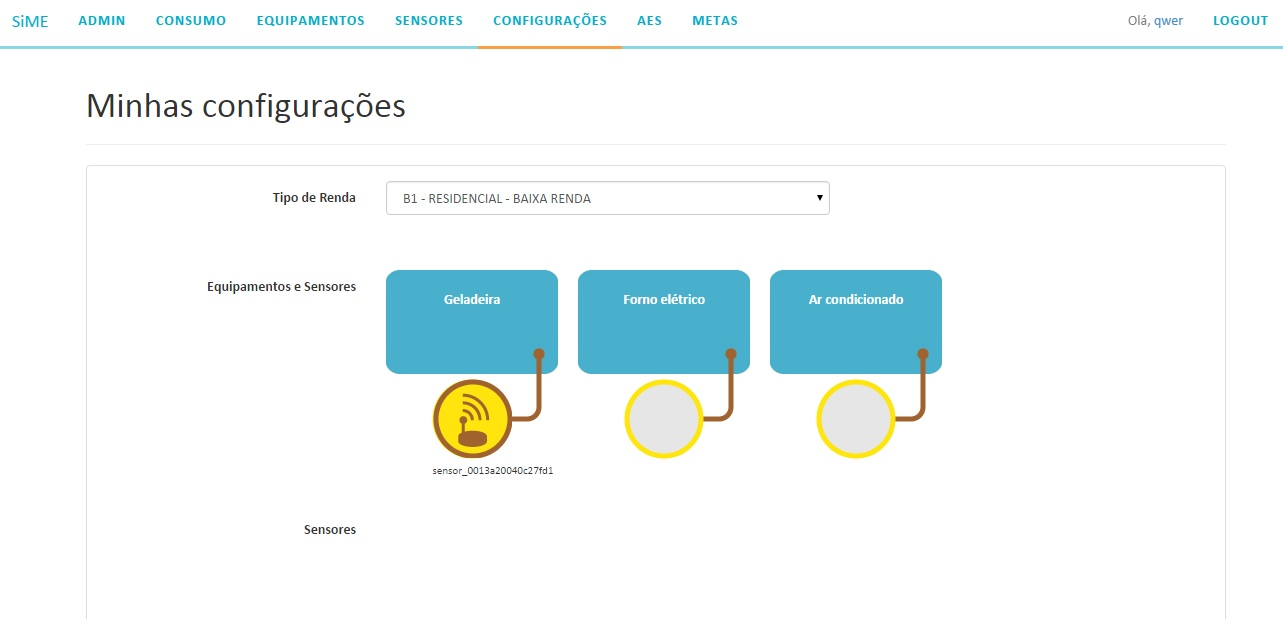
\includegraphics[width=1\textwidth]{figuras/configuracoes.jpg}
\caption{\label{fig:telas-config} Configurações}
\end{figure}

%\subsubsection{Consumo}

\subsubsection{Visualização dos dados medidos}
\begin{figure}[H]
\centering
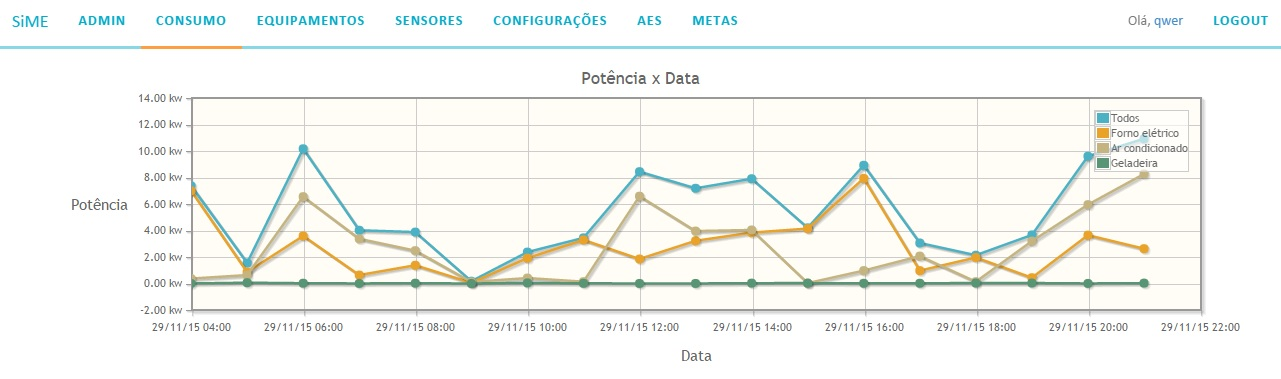
\includegraphics[width=1\textwidth]{figuras/consumo.jpg}
\caption{\label{fig:telas-grafico} Gráfico de consumo}
\end{figure}


\subsection{Heroku}

Heroku é uma plataforma que oferece serviços em cloud. Esse serviço é usado no projeto para hospedar a aplicação desenvolvida. A grande vantagem do serviço  é o fato de ser gratuito com algumas limitações, que não se tornaram empecilhos para o trabalho, e retirar a responsabilidade do módulo coordenador de segurar a aplicação.